\begin{frame}
    \frametitle{On cherche des réponses}
    \alert{Who was the wife of Louis Pasteur?}
    \begin{figure}
        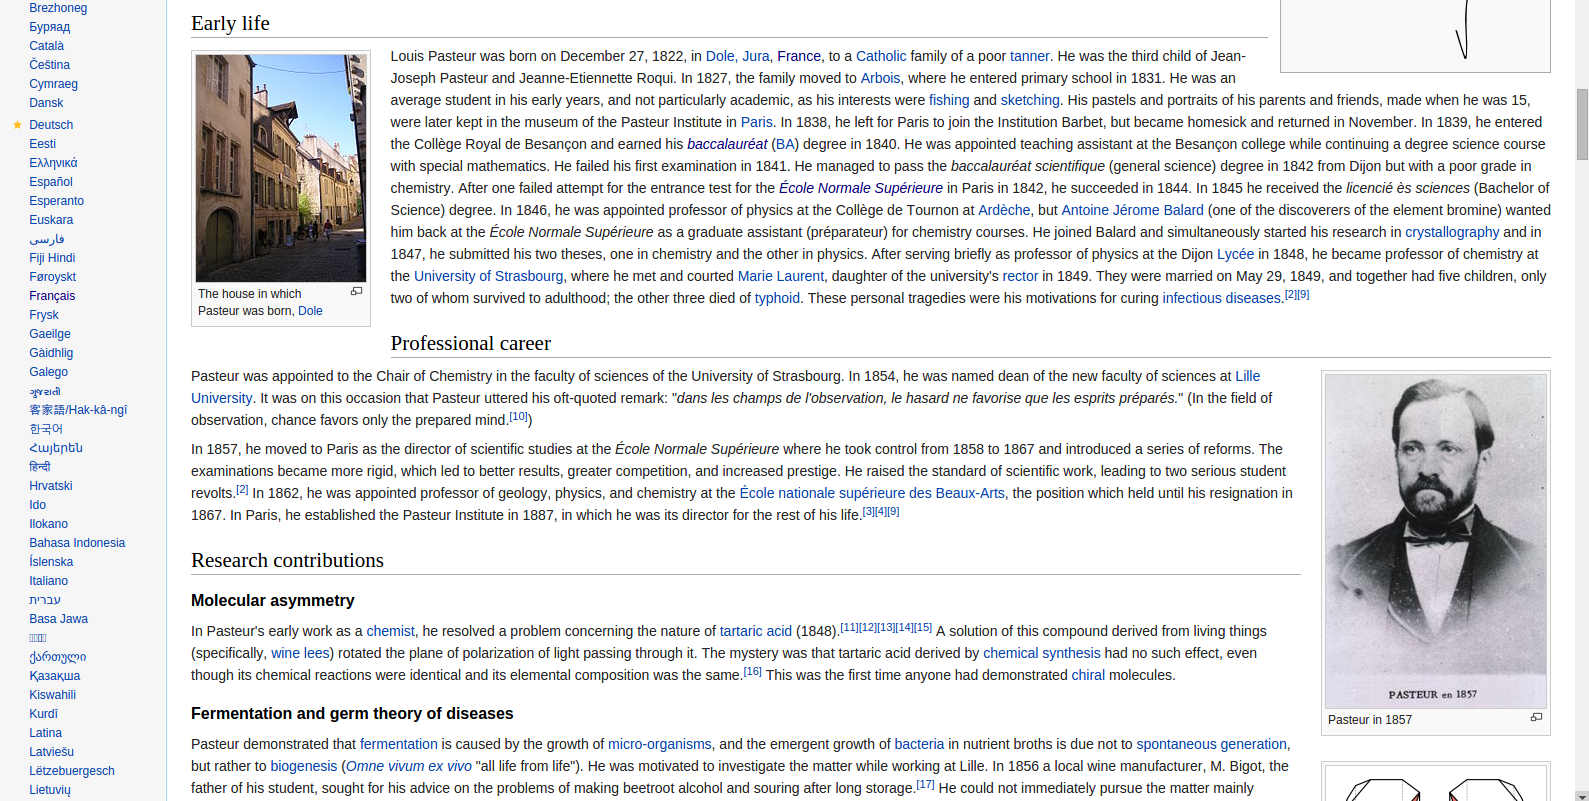
\includegraphics[width=\textwidth]{pasteurWiki.png}
    \end{figure}
\end{frame}

\begin{frame}
    \frametitle{Outils existants}
    \begin{tabular}{ll}
        WolframAlpha & Marie Pasteur\\
        Google & Article Wikipedia sur Marie Pasteur\\
        Bing & Article Wikipedia Louis Pasteur\\
        Yahoo & Page d'answers.com contenant la question
    \end{tabular}
\medbreak
\alert{Logiciels propriétaire, parfois mauvais...}
\end{frame}

\begin{frame}
    \frametitle{Platypus}
    \begin{center}
        \url{http://askplatyp.us}
        
        \bigskip
        
        
\includegraphics[width=0.6\linewidth]{figures/platypus.pdf}
    \end{center}
\end{frame}

\begin{frame}
    \frametitle{Platypus ?}
    \begin{itemize}
        \item<1-> \alert{Open-source}
        \item<2-> \alert{Modulaire}
        \item<3-> \alert{Anglais} pour l'instant
        \item<4-> \alert{Connaissance générale} et math
    \end{itemize}
\end{frame}

\begin{frame}
    \begin{center}
        \Huge Et la démo !
    \end{center}
\end{frame}

\begin{frame}[plain]
    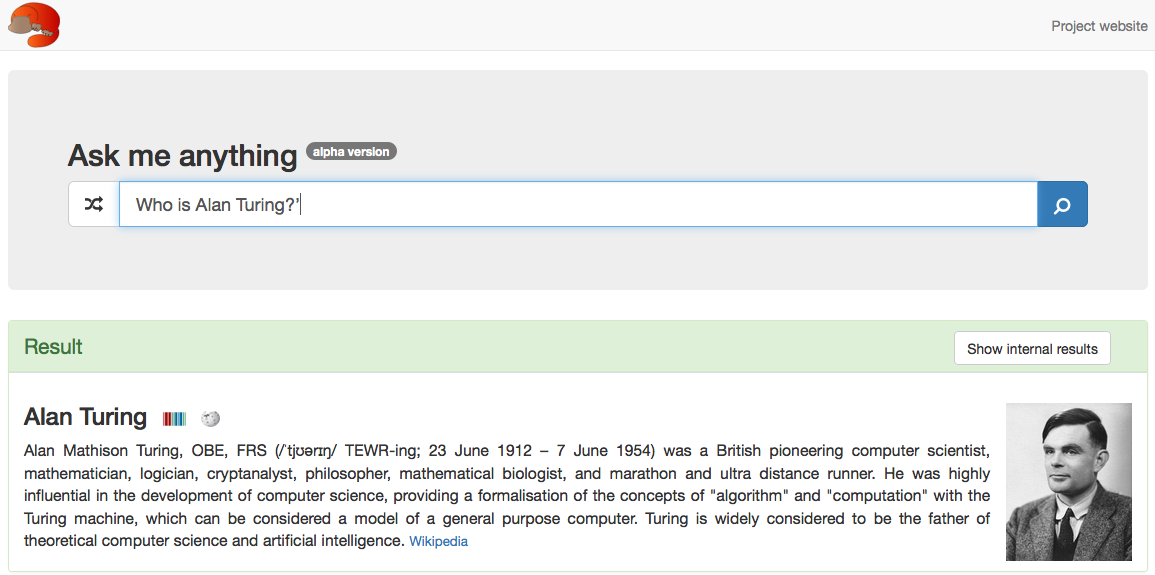
\includegraphics[width=\linewidth]{figures/demo-whoIsAlanTuring.png}
\end{frame}

\begin{frame}[plain]
    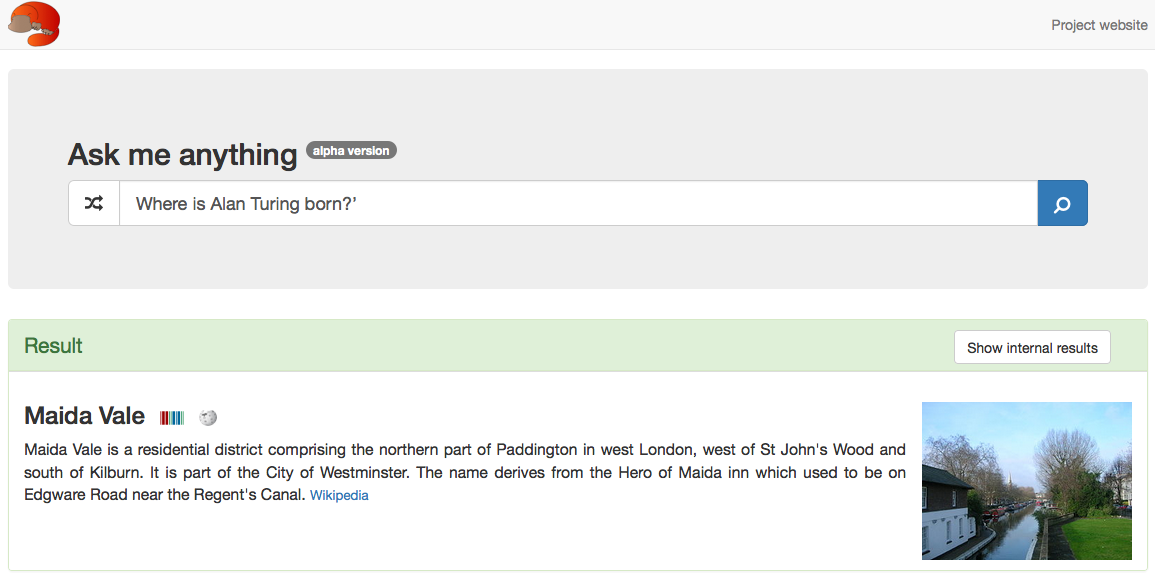
\includegraphics[width=\linewidth]{figures/demo-whenIsAlanTuringBorn.png}
\end{frame}

\begin{frame}[plain]
    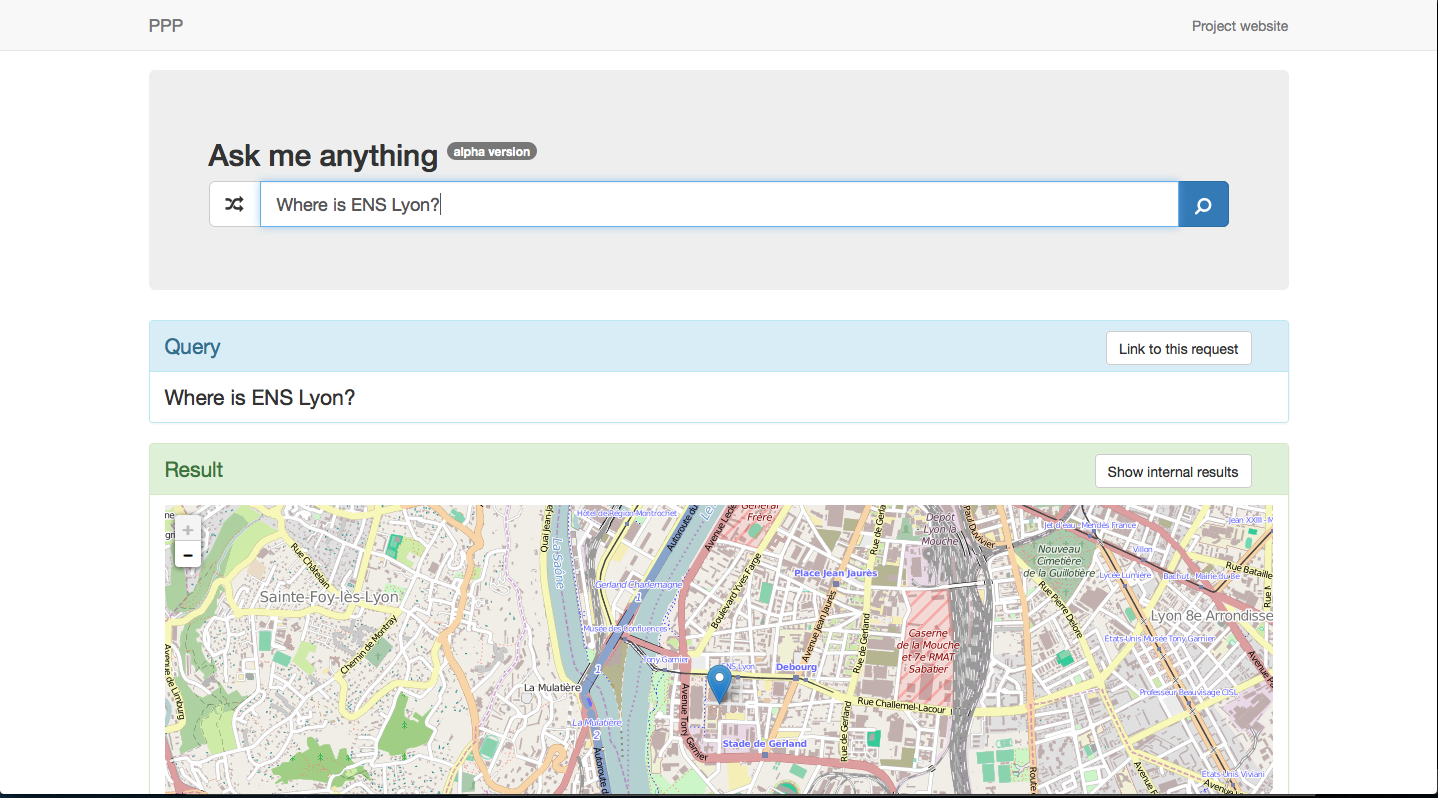
\includegraphics[width=\linewidth]{figures/demo-whereIsEnsLyon.png}
\end{frame}
